% Issue #81, part "Results and discussion"; owner: vks-g. Input from reports/phase2/main.tex.
% Numbers: results/metrics/fd001_final_test*.{json,csv}, fd001_ml_capped_test*.{json,csv} and
% fd001_final_comparison.csv (notebooks/phase2/15_final_comparison.ipynb, #71);
% fd001_validation_*.{csv,json} (#72); fd001_cv_*.json and fd001_ml_capped_cv.json (CV column).
% Table: tables/final_results.tex, generated by scripts/prepare_results_tables.py.
% Figure: results/figures/fd001_final_predictions.png (#71).

\section{Results and Discussion}
\label{sec:results}

Every model was frozen at one commit and scored once on the 100 official
FD001 test engines (Section~\ref{sec:validation}). Table~\ref{tab:final_results}
puts each model's cross-validated selection RMSE next to its test scores, and
Fig.~\ref{fig:final_predictions} shows the predictions engine by engine. This
section answers the three questions of Section~\ref{sec:introduction}, then
discusses what matters more than the model, how well cross-validation
predicted the test, and the limits of the evidence.

\begin{table*}[t]
\centering
\caption{Every model trained with the cap of 125. CV: selection RMSE in
cross-validation at seed 42 (mean over 3 folds, held-out cycles with true RUL
$\leq130$). It scores every held-out cycle rather than each engine's last
cycle, so compare its ranking with the test, not its level. Official test: RMSE
and NASA score as mean $\pm$ s.d.\ over 5 seeds for the networks and one run
for the ML baselines, and RMSE by life stage at the last cycle: late
($y\leq50$, 33 engines), mid ($50<y\leq100$, 34) and early ($y>100$, 33).}
\label{tab:final_results}
\footnotesize
% Generated by scripts/prepare_results_tables.py from the cross-validation results
% (fd001_cv_*.json, fd001_ml_capped_cv.json) and the #71 test predictions. Do not edit by hand.
\begin{tabular}{@{}lcccccc@{}}
\hline
 & CV & \multicolumn{5}{c}{Official test} \\
Model & $\mathrm{RMSE}_{\leq130}$ & RMSE & NASA score & Late & Mid & Early \\
\hline
Hybrid B, two-stage & 14.38 & 15.18 $\pm$ 0.55 & 356 $\pm$ 22 & 6.16 & 16.53 & 19.38 \\
Hybrid A, gated & 16.81 & 15.40 $\pm$ 0.46 & 488 $\pm$ 116 & 5.08 & 20.57 & 16.01 \\
Transformer & 15.59 & 15.60 $\pm$ 0.35 & 443 $\pm$ 49 & 6.44 & 21.06 & 15.42 \\
XGBoost, engineered & 14.49 & 15.71 & 389 & 6.27 & 18.22 & 19.14 \\
Temporal CNN & 17.24 & 15.83 $\pm$ 0.55 & 414 $\pm$ 66 & 7.58 & 19.28 & 17.73 \\
LSTM & 15.78 & 15.95 $\pm$ 0.33 & 499 $\pm$ 39 & 5.50 & 21.38 & 16.38 \\
Random Forest, engineered & 15.16 & 16.21 & 412 & 7.39 & 18.14 & 20.05 \\
XGBoost, raw & 18.90 & 17.58 & 575 & 13.63 & 17.59 & 20.78 \\
Elastic Net, engineered & 18.94 & 17.80 & 481 & 17.51 & 15.93 & 19.80 \\
Random Forest, raw & 19.00 & 18.42 & 578 & 14.13 & 17.54 & 22.63 \\
Elastic Net, raw & 20.97 & 22.44 & 1{,}269 & 23.68 & 18.08 & 25.08 \\
\hline
\end{tabular}

\end{table*}

\begin{figure*}[t]
\centering
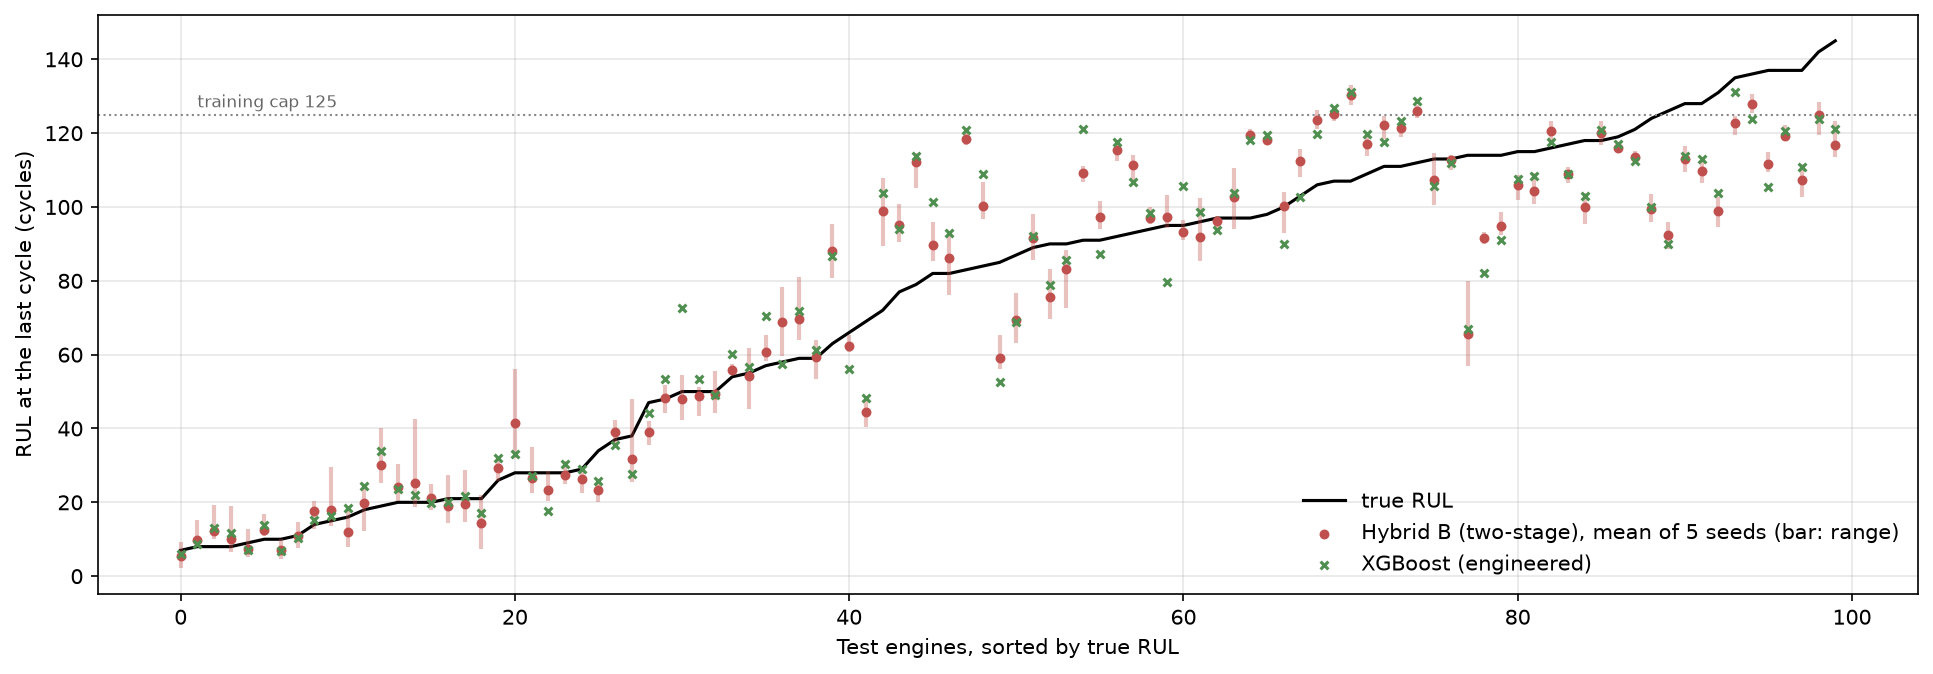
\includegraphics[width=\textwidth]{../../results/figures/fd001_final_predictions.png}
\caption{Each official test engine's prediction at its last cycle, sorted by
true RUL: Hybrid~B (mean of five seeds, bar: range over seeds) and XGBoost on
engineered features. Both follow the true RUL closely near failure. Above the
training cap of 125, both stop rising, so every model trained with the cap
predicts early there.}
\label{fig:final_predictions}
\end{figure*}

\subsection{Sequence Models against Engineered Features}
With the same capped target and selection metric, the three encoders score
15.60 (Transformer), 15.83 (temporal CNN) and 15.95 (LSTM), and XGBoost on
the engineered features scores 15.71. The comparison fixed in advance, the
Transformer against XGBoost, is a tie ($-0.11$ cycles, interval $-2.42$ to
$+2.26$). Our LSTM reproduces the closest published protocol: Gupta's LSTM,
with the same cap, window, uncapped test labels and five seeds, scored
$15.97\pm0.45$~\cite{Gupta2026auditing}, against our $15.95\pm0.33$.

So on FD001, learning from raw sensor windows does not beat engineered
features with boosted trees, but it matches them without the features. The
life stages show where this matters. Near failure, where maintenance is
decided, every network scores 5.1 to 7.6 cycles, as accurate as the trees on
engineered features. The ML models on raw inputs are two to four times worse
there (13.6 to 23.7). The sequence models learn from raw windows what the trees
need the Phase~1 features for. Over all engines, the three encoders are 1.6 to
2.0 cycles better than the best ML model on raw inputs (XGBoost, 17.58),
though their bootstrap intervals overlap (Table~\ref{tab:validation_models}).
In mid life the three encoders and Hybrid~A are weakest (19.3 to 21.4), and the
encoders predict late on average, by 9.8 to 12.9 cycles against 6.3 to 7.3 for
the trees on engineered features. Early in life the networks and these trees
all predict early on average, from 5.7 cycles (Transformer) to 10.5 (Random
Forest), because none of them predicts much above the cap. The Transformer is the most accurate there
(15.42).

\subsection{Which Encoder}
Cross-validation ranked the Transformer (15.59) and the LSTM (15.78) ahead of
the temporal CNN (17.24). On the test, the three lie within 0.35 cycles of
each other, about the size of their seed spread (0.33 to 0.55). No way of
reading the window wins on FD001: recurrence, dilated convolution and attention reach the
same accuracy on 30-cycle windows of 100 training engines. They differ in
their errors rather than their accuracy. The LSTM and the Transformer predict
late on average (by 2.65 and 2.85 cycles), which the NASA score punishes
(499 and 443). The temporal CNN's mean error is smaller (1.04), and so is its
score (414).

\subsection{Do the Hybrids Add Value?}
Hybrid~B has the lowest test RMSE ($15.18\pm0.55$) and the lowest NASA score
($356\pm22$, against 389 for XGBoost), and its mean error ($-0.78$ cycles) is
the smallest of the five networks. Its mid-life gain over XGBoost ($-1.69$,
interval $-3.25$ to $-0.25$) is the one place where the LSTM embeddings seem to
help. Under the value test fixed in advance, however, both hybrids give null
results on the official test (Table~\ref{tab:validation_paired}). Hybrid~B is
$-0.53$ cycles from XGBoost (interval $-1.45$ to $+0.38$). Hybrid~A is $-0.54$
from the LSTM ($-3.35$ to $+2.24$), and its cross-validated pass on seed spread
does not carry over: on the test it varies more than the LSTM (0.46 against
0.33), and its NASA score varies most of all ($488\pm116$). On FD002 and
FD004, the gated hybrid and the LSTM are also within half a cycle of each
other (Table~\ref{tab:multi_regime_test}).

We therefore report that neither hybrid demonstrably adds value on FD001.
Three points qualify this null result. First, it is a null result and not a
loss: neither hybrid has a higher mean error than its best branch, in
cross-validation or on the test. Second, the test has limited power. The
narrowest paired interval, Hybrid~B against XGBoost, spans 1.8 cycles, so a
gain like Chen et al.'s 0.6 cycles from adding features to an LSTM on
FD001~\cite{Chen2021machine} could not be detected with 100 test engines.
Third, the null result is informative. The engineered rolling features
already carry most of the degradation signal that the LSTM finds in a
30-cycle window, so on FD001 there is little left for fusion to add.

\subsection{What Matters More than the Model}
Three pipeline choices move the error by more than any choice of model. The
training cap is the largest: trained uncapped, every model is 7 to 15 cycles
worse on the test, and the uncapped encoders vary by 3.5 to 5.0 cycles across
seeds. Most of the improvement since Phase~1 comes from the cap. Phase~1's
Random Forest went from 27.55 uncapped to 16.21 capped, while the best Phase~2
model, at 15.18, improves on the capped Random Forest by about one cycle,
within the test's noise. The difference is that the cap is now chosen from
training engines (Section~\ref{sec:target_selection}). The inputs come next:
every ML model is 1.9 to 4.6 cycles worse on raw inputs than on engineered
ones. On the multi-regime subsets, per-regime scaling improved the LSTM by
1.30 (FD002) and 3.20 cycles (FD004) in cross-validation
(Section~\ref{sec:validation}).

Seed variation is also large. Averaging each engine's prediction over the five
seeds gives 14.71 for Hybrid~B, 14.98 for the temporal CNN and 15.08 for
Hybrid~A, lower than any single-seed mean. Seed averaging was not part of the
frozen protocol, so we report it as an observation, not as a result.

\subsection{Cross-Validation against the Test}
Over all eleven models in Table~\ref{tab:final_results}, the cross-validated
ranking agrees with the test ranking (Spearman rank correlation 0.81). Among
the seven best models, it does not (0.25). Hybrid~A was sixth of these seven
in cross-validation and second on the test, and XGBoost went from second to
fourth. Cross-validation separates
good models from poor ones, but no evaluation on 100 engines can order models
that are within a cycle of each other. This is why every comparison was fixed
from cross-validation before the test was read, rather than chosen from test
scores.

\subsection{Limits}
The evidence has five limits. (i)~One test set of 100 engines: the best
models' bootstrap intervals are 4 to 5 cycles wide. (ii)~The networks ran at five seeds
and the ML baselines at one, so the seed spread of the ML models is unknown.
(iii)~Every setting was tuned at seed 42, and a network's cross-validated score
moves by up to 2 cycles between seeds. (iv)~The cap rule was designed after the
Phase~1 test result at a cap of 125 was known
(Section~\ref{sec:target_selection}). (v)~The main comparison covers FD001 only.
FD002 and FD004 reused the FD001 settings, and a cap of 150 was not tried
there.
